\documentclass[12pt,a4paper]{article}
\usepackage[utf8]{vietnam}
\usepackage[a4paper,margin=2.5cm]{geometry}
\usepackage{amsmath,amssymb,amsthm,booktabs,array}
\usepackage{graphicx,float,hyperref}
\usepackage{placeins}
\hypersetup{colorlinks=true,linkcolor=blue,citecolor=blue,urlcolor=blue}
\newtheorem{definition}{Định nghĩa}[section]
\newtheorem{proposition}{Mệnh đề}[section]
\newtheorem{remark}{Nhận xét}[section]
\newcommand{\OPT}{\texttt{OPT}}
\newcommand{\FEAS}{\texttt{FEASIBLE}}
\newcommand{\CycleCount}{48}
\newcommand{\ProductCount}{448}
\newcommand{\ComparisonCount}{496}
\newcommand{\PairedOpt}{494}
\newcommand{\UnresolvedCount}{2}
\newcommand{\WitnessCount}{992}
\newcommand{\CycleFirst}{3}
\newcommand{\CycleLast}{50}
\newcommand{\ProductFirst}{3}
\newcommand{\ProductLast}{10}
\newcommand{\ProductMFirst}{3}
\newcommand{\ProductMLast}{10}
\newcommand{\CycleClauseMedian}{12.58}
\newcommand{\CycleTimeRatio}{1.000}
\newcommand{\CxCTimeRatio}{1.103}
\newcommand{\CxCTotalTimeRatio}{2.48}
\newcommand{\CoCTimeRatio}{1.120}
\newcommand{\CoCTotalTimeRatio}{1.72}
\newcommand{\CoPTimeRatio}{1.112}
\newcommand{\CoPTotalTimeRatio}{1.41}
\newcommand{\CoronaPathMatches}{64}
\newcommand{\CoronaPathCount}{64}

\title{Phương pháp SAT và ILP\\
cho bài toán $L(2,1)$-labeling\\[0.5em]
{\large Mô hình, phá đối xứng và thực nghiệm trên các họ đồ thị}}
\author{Bản thảo nghiên cứu}
\date{Tháng 9 năm 2026}
\begin{document}
\maketitle
\begin{abstract}
Nghiên cứu xây dựng công cụ giải chính xác bài toán tối thiểu hóa span của phép
gán nhãn $L(2,1)$ trên đồ thị. Phương pháp SAT dùng order encoding và tìm kiếm
trên khoảng cận dưới--cận trên; hai mô hình ILP được triển khai để đối chiếu.
Báo cáo trình bày tính tương đương của mã hóa, điều kiện hợp lệ của phá đối xứng,
và cách phân biệt nghiệm khả thi với kết luận tối ưu. Thực nghiệm SAT gồm
\CycleCount{} chu trình và \ProductCount{} đồ thị tích, mỗi đồ thị chạy hai
cấu hình Baseline/Symmetry. Có \PairedOpt{} trên \ComparisonCount{} cặp cùng
xác nhận tối ưu với span bằng nhau; \UnresolvedCount{} cặp còn lại chưa xác
nhận tối ưu trong budget. Toàn bộ \WitnessCount{} labeling đã lưu được kiểm
tra lại, và hai CNF được đếm tại cùng span. Chỉ chu trình được cố định gốc;
các họ product sử dụng thứ tự dựa trên phản xạ hoặc không thêm đối xứng riêng.
Lợi ích về kích thước và thời gian thay đổi theo họ; một lượt chạy chưa đủ
để kết luận về độ ổn định của cải thiện hiệu năng. ILP được trình bày ở mức
mô hình, chưa có đối chứng hiệu năng mới trong hai lượt thực nghiệm này.
\end{abstract}
\clearpage
\tableofcontents
\clearpage
\section{Bài toán và phạm vi nghiên cứu}
\subsection{Định nghĩa và quy ước}
Cho đồ thị đơn, vô hướng, không có khuyên $G=(V,E)$. Đặt
\[
D_2(G)=\{\{u,v\}\subseteq V:d_G(u,v)=2\}.
\]
Các cặp trong $D_2(G)$ là cặp không có thứ tự và không bao gồm cạnh của $G$.
Với hai số nguyên $h\geq k\geq 1$, một phép gán nhãn $L(h,k)$ là ánh xạ
$f:V\to\mathbb Z_{\geq0}$ thỏa
\begin{align}
|f(u)-f(v)|&\geq h &&\forall\{u,v\}\in E,\\
|f(u)-f(v)|&\geq k &&\forall\{u,v\}\in D_2(G).
\end{align}
Span của $f$ là $\max_v f(v)-\min_v f(v)$, và $\lambda_{h,k}(G)$ là
span nhỏ nhất. Với đồ thị rỗng, quy ước span bằng 0. Khi $h\geq k$, cách định
nghĩa qua khoảng cách đúng bằng 2 tương đương với điều kiện trên hai đỉnh có
chung lân cận; nếu xét $h<k$ phải phân biệt hai quy ước này \cite{calamoneri}.

Do các ràng buộc chỉ phụ thuộc hiệu nhãn, phép tịnh tiến
$f'(v)=f(v)-\min_u f(u)$ bảo toàn tính hợp lệ và span. Vì vậy, có thể dùng
miền nhãn $\{0,\ldots,s\}$ để kiểm tra span không quá $s$. Có $s+1$ nhãn
khả dụng, nhưng không bắt buộc dùng hết chúng. Các đỉnh cách nhau hơn 2 bước
được phép nhận cùng nhãn.

Phần mô hình SAT có tham số $h,k$; các solver tối ưu, cận, thuật toán tham lam
và benchmark trong phiên bản này tập trung vào $h=2,k=1$. Không suy rộng kết
quả thực nghiệm thành kết quả cho mọi $L(h,k)$.

\subsection{Cơ sở lý thuyết và mục tiêu}
Bài toán bắt nguồn từ phân bổ tần số: các trạm gần nhau cần cách biệt tần số
đủ lớn. Griggs và Yeh đặt nền tảng cho $L(2,1)$, nghiên cứu các họ cơ bản,
các cận theo bậc và tính NP-đầy đủ của phiên bản quyết định \cite{griggs}.
Survey của Calamoneri tổng hợp thuật toán, kết quả độ phức tạp và công thức
trên các họ đồ thị \cite{calamoneri}.

Trên cây không tầm thường, $\lambda_{2,1}(T)\in\{\Delta+1,\Delta+2\}$.
Hasunuma và cộng sự xây dựng thuật toán tuyến tính dùng quy hoạch động,
khả năng thay thế nhãn và mạng luồng thu gọn \cite{hasunuma}. Project chưa
triển khai thuật toán này; đây là nền tảng cho đối chứng chuyên biệt trong
nghiên cứu tiếp theo.

Mục tiêu của công cụ là giải từng instance bằng mô hình chính xác, đánh giá
chi phí mã hóa và tìm kiếm, kiểm tra nhãn độc lập, và thu thập bằng chứng tính
toán có thể truy nguyên. Các họ đã có công thức giúp kiểm tra tính đúng đắn;
các họ khác giúp khảo sát quy luật và xây dựng giả thuyết. Việc khẳng định một
kết quả mới đòi hỏi đối chiếu tài liệu riêng, không chỉ dựa vào bảng thực nghiệm.

\subsection{Các họ đồ thị}
Ngoài chu trình $C_n$, đồ thị đầy đủ $K_n$ và siêu lập phương $Q_d$, benchmark
xét ba họ Cartesian
\[
 C_n\mathbin{\square} C_m,\qquad C_n\mathbin{\square} P_m,\qquad P_n\mathbin{\square} P_m,
\]
và bốn họ Corona
\[
 C_n\circ C_m,\quad C_n\circ P_m,\quad P_n\circ C_m,\quad P_n\circ P_m.
\]
Tích Cartesian có đỉnh $(u,a)$ và cạnh khi một tọa độ giữ nguyên còn tọa độ
kia là một cạnh trong đồ thị thành phần. Tích Corona $G\circ H$ gồm một bản
sao $G$, một bản sao riêng của $H$ cho mỗi đỉnh $u\in V(G)$, và nối $u$ với
mọi đỉnh của bản sao tương ứng \cite{frucht}. Nếu $G,H$ có lần lượt $n,m$
đỉnh thì
\[
|V(G\circ H)|=n(m+1),\qquad
|E(G\circ H)|=|E(G)|+n|E(H)|+nm.
\]
Phiên bản hiện tại xét Corona thông thường; không gộp với edge corona hay
neighborhood corona.

Họ $GP(n,k)$ trong code có cạnh $u_iu_{i+1}$, $u_iv_i$, $v_iv_{i+k}$,
với chỉ số modulo $n$ và $1\leq k<n/2$. Đồ thị có $2n$ đỉnh, $3n$ cạnh.
Cần phân biệt họ này với $GPG(n)$ trong bài của Huang và cộng sự
\cite{huang}: bài báo dùng hai chu trình độ dài $n$ nối bởi một matching tùy
ý. Khi $\gcd(n,k)=1$, chu trình bên trong của $GP(n,k)$ liên thông và đồ thị
thuộc lớp đó; khi $\gcd(n,k)>1$, các cạnh bước $k$ tạo nhiều chu trình.
Quét các giá trị $k$ cũng không liệt kê mọi matching của $GPG(n)$.
Do đó, sweep $GP(n,k)$ không phải kiểm chứng toàn bộ giả thuyết Georges--Mauro
trên $GPG(n)$.

\section{Các mô hình chính xác}
\subsection{SAT với order encoding}
Cho span ứng viên $s\geq0$. Với mỗi đỉnh $v$ và $0\leq i<s$, tạo biến
\[
 x_{v,i}\Longleftrightarrow [f(v)\leq i].
\]
Dùng hằng $x_{v,-1}=\bot$ và $x_{v,s}=\top$. Các mệnh đề đơn điệu là
\begin{equation}
 \neg x_{v,i}\lor x_{v,i+1},\qquad 0\leq i<s-1.
\end{equation}
Khi đó $f(v)=a$ tương đương $x_{v,a}\land\neg x_{v,a-1}$. Với cặp đỉnh
cần cách biệt ít nhất $d$, loại mỗi cặp nhãn $(a,b)$ có $|a-b|<d$ bằng
\begin{equation}\label{eq:forbidden}
 \neg x_{u,a}\lor x_{u,a-1}\lor\neg x_{v,b}\lor x_{v,b-1}.
\end{equation}
Chọn $d=h$ cho cạnh và $d=k$ cho cặp khoảng cách hai. Các hằng tại biên được
rút gọn. Với $s=0$, một ràng buộc cách biệt dương sinh mệnh đề rỗng, đúng với
tính bất khả thi khi mọi đỉnh chỉ có thể nhận nhãn 0.

\begin{proposition}
Nếu chưa thêm ràng buộc đối xứng, CNF ở trên khả thỏa khi và chỉ khi tồn tại
một $L(h,k)$-labeling có span không quá $s$.
\end{proposition}
\begin{proof}
Một labeling trong $[0,s]$ xác định các biến ngưỡng, thỏa đơn điệu và không
chọn bất kỳ cặp nhãn bị cấm nào. Ngược lại, một dãy biến ngưỡng đơn điệu xác
định duy nhất một nhãn: chỉ số đầu tiên có giá trị đúng, hoặc $s$ nếu mọi
biến đều sai. Nếu hai nhãn vi phạm một điều kiện cách biệt, mệnh đề
\eqref{eq:forbidden} tương ứng sẽ sai. Do vậy mọi labeling giải mã đều hợp lệ.
Tịnh tiến nhãn nhỏ nhất về 0 cho phép áp dụng kết luận với định nghĩa span.
\end{proof}

Trước khi rút gọn đỉnh cố định, số biến là $|V|s$. Với $L(2,1)$, số mệnh đề
được sinh trước khi rút gọn hoặc loại trùng là
\begin{equation}
 |V|\max(s-1,0)+|E|A(s)+|D_2(G)|(s+1),
 \quad A(s)=\begin{cases}1&s=0,\\3s+1&s\geq1.\end{cases}
\end{equation}
Các số đếm trong kết quả là số biến encoder cấp phát và số mệnh đề truyền
cho solver, không phải số còn lại sau preprocessing nội bộ của SAT solver.

\subsection{ILP dạng assignment}
Cho $U$ là cận trên từ một labeling tham lam hợp lệ. Để tránh trùng ngữ nghĩa
với biến ngưỡng SAT, ký hiệu biến nhị phân ILP là $y_{v,a}$:
$y_{v,a}=1$ khi và chỉ khi $f(v)=a$. Mô hình tổng quát là
\begin{align}
 \min\quad &\ell_{\max}\\
 \sum_{a=0}^{U}y_{v,a}&=1 &&\forall v\in V,\label{eq:assignment}\\
 y_{u,a}+y_{v,b}&\leq1
 &&\forall\{u,v\}\in E,\ |a-b|<h,\\
 y_{u,a}+y_{v,b}&\leq1
 &&\forall\{u,v\}\in D_2(G),\ |a-b|<k,\\
 \sum_{a=0}^{U}a\,y_{v,a}&\leq\ell_{\max} &&\forall v\in V,\\
 y_{v,a}&\in\{0,1\},\quad \ell_{\max}\in\{0,\ldots,U\}.
\end{align}
Trong hai ràng buộc cấm, $a,b\in\{0,\ldots,U\}$. Ràng buộc
\eqref{eq:assignment} chọn đúng một nhãn. Vì mô hình không ép một đỉnh tùy ý
về 0, tối thiểu hóa $\ell_{\max}$ đạt span tối ưu nhờ bất biến tịnh tiến.
Trong triển khai $h=2,k=1$, điều kiện khoảng cách hai chỉ cần cấm nhãn bằng nhau.
Số biến là $|V|(U+1)+1$, số ràng buộc là
\[
2|V|+(3U+1)|E|+(U+1)|D_2(G)|.
\]

\begin{remark}[Quy ước nhãn bắt đầu từ 1]
Nếu dùng miền nhãn $\{1,\ldots,U'\}$ như một số cách viết assignment, tối ưu
của biến nhãn lớn nhất bằng $\lambda_{h,k}(G)+1$ trên đồ thị không rỗng.
Khi chuyển sang quy ước bắt đầu từ 0 phải dùng $U=U'-1$ và báo cáo
$\lambda=\ell_{\max}-1$. Không được đồng nhất số nhãn khả dụng với span.
\end{remark}

\subsection{ILP dạng Big-M}
Dùng biến nguyên $0\leq f_v\leq U$, $0\leq\ell_{\max}\leq U$ và
$f_v\leq\ell_{\max}$. Với mỗi cặp cần cách biệt ít nhất $d$, thêm biến
$z_{uv}\in\{0,1\}$ và
\begin{align}
 f_u-f_v&\geq d-Mz_{uv},\\
 f_v-f_u&\geq d-M(1-z_{uv}).
\end{align}
Chọn $M=U+\max(h,k)$ đủ để vô hiệu hóa bất đẳng thức không được chọn vì
$-U\leq f_u-f_v\leq U$. Mục tiêu vẫn là $\min\ell_{\max}$.
Triển khai $L(2,1)$ dùng $M=U+2$. Số biến là
$|V|+1+|E|+|D_2(G)|$; số ràng buộc là
$|V|+2|E|+2|D_2(G)|$.

Cả hai mô hình dùng nghiệm tham lam làm MIP start. Assignment loại cặp nhãn
trực tiếp nhưng kích thước tăng theo $U$; Big-M thường gọn hơn nhưng có hệ số
phụ thuộc cận trên. Đây là lý do cần thực nghiệm đối chứng, chưa phải kết luận
một mô hình luôn nhanh hơn mô hình còn lại.

\section{Tìm kiếm span và phá đối xứng}
\subsection{Cận và bất biến tìm kiếm}
Với đồ thị có ít nhất một cạnh, cận dưới cho $L(2,1)$ là
$L=\Delta(G)+1$. Thật vậy, $\Delta$ lân cận của một đỉnh bậc cực đại phải
nhận nhãn đôi một khác nhau: chúng kề nhau hoặc cách nhau hai bước. Chúng
cũng không được nhận nhãn của đỉnh trung tâm hay nhãn chênh 1 với nó. Miền
có span $\Delta$ không đủ chứa các nhãn đó. Đồ thị không có cạnh có span 0.

Thuật toán tham lam duyệt một thứ tự đỉnh cố định, chọn số nguyên không âm
nhỏ nhất không vi phạm các đỉnh đã gán. Gọi $U$ là span của nghiệm này;
validator kiểm tra lại trước khi dùng làm incumbent. Bất biến là
\[
 L\leq\lambda_{2,1}(G)\leq U,
\]
trong đó phía trên luôn có một labeling cụ thể đi kèm.

Tìm kiếm tuyến tính thử $s=U-1$. Tìm kiếm hybrid trong phiên bản hiệu chỉnh
thử $s=\lfloor(L+U)/2\rfloor$. Nếu SAT, giải mã và chuẩn hóa labeling rồi
hạ $U$ về span thực tế. Nếu UNSAT, đặt $L=s+1$. Dừng khi $L=U$ và trả
\OPT. Không cần giải lặp lại một span đã có kết luận. Mỗi lần thử xây CNF
và tạo solver mới; phiên bản này chưa phải SAT gia tăng qua các span.

\begin{proposition}
Nếu cận khởi tạo hợp lệ, mã hóa tương đương và các ràng buộc đối xứng bảo toàn
khả thỏa, thuật toán kết luận \OPT{} chỉ khi incumbent là tối ưu.
\end{proposition}
\begin{proof}
SAT cung cấp cận trên hợp lệ. UNSAT ở $s$ loại mọi span không quá $s$ do tính
đơn điệu của miền nhãn. Hai cập nhật giữ bất biến; khi hai cận gặp nhau,
giá trị tối ưu bị kẹp bằng span incumbent.
\end{proof}
Timeout không phải UNSAT và không được nâng cận dưới. Nếu hết thời gian khi
$L<U$, trả \FEAS{} cùng incumbent; khi $L=U$ ngay từ cận tham lam thì có
thể trả \OPT{} mà không cần gọi SAT. Khi đó số biến và mệnh đề có thể để trống.

\subsection{Điều kiện đúng của phá đối xứng}
Tịnh tiến chỉ bảo đảm \emph{có một đỉnh} nhận nhãn 0. Để cố định một đỉnh
đã chọn $v_0$ về 0, cần thêm lập luận về cấu trúc đồ thị.
\begin{proposition}
Nếu $G$ là vertex-transitive, có thể thêm $f(v_0)=0$ mà không làm thay đổi
span tối ưu hoặc tính khả thỏa của bài toán span không quá $s$.
\end{proposition}
\begin{proof}
Chuẩn hóa một labeling hợp lệ để một đỉnh $w$ có nhãn 0. Tính vertex-transitive
cho một tự đẳng cấu đưa $v_0$ đến $w$. Hợp thành labeling với tự đẳng cấu đó
bảo toàn mọi khoảng cách và đưa nhãn tại $v_0$ về 0.
\end{proof}

Riêng với $C_n$, chọn $t$ sao cho $f(t)=\min_i f(i)$ và đặt
\[
 g(i)=f((i+t)\bmod n)-f(t).
\]
Phép quay bảo toàn khoảng cách và phép tịnh tiến bảo toàn hiệu nhãn, nên
$g$ hợp lệ, $g(0)=0$ và có cùng span với $f$. Cơ sở là tự đẳng cấu quay
của chu trình, không phải chỉ việc các đỉnh có cùng bậc.

Trong phạm vi thí nghiệm này, chỉ áp dụng cố định gốc cho chu trình $C_n$.
Mệnh đề tổng quát trên là cơ sở lý thuyết, không có nghĩa triển khai cố định
gốc trên mọi họ vertex-transitive. Các họ khác chỉ dùng những thứ tự được
liệt kê trong bảng dưới. Các biến ngưỡng của đỉnh cố định không cần cấp phát; một đỉnh cố định
loại $s$ biến. Các ràng buộc liên quan được thay hằng và rút gọn trước khi gọi
solver. Đây là giảm kích thước CNF do cố định nhãn; việc chỉ thêm một bất đẳng
thức thứ tự có thể làm tăng số mệnh đề.

Phiên bản hiện tại áp dụng cùng một tiền xử lý cho cả Baseline và Symmetry:
bỏ mệnh đề hằng đúng, bỏ bản sao và lan truyền đơn vị đến điểm cố định.
Nếu có mệnh đề đơn $\ell$, mọi mệnh đề chứa $\ell$ được thỏa mãn; trong
các mệnh đề còn lại có thể bỏ $\neg\ell$. Giữ lại mệnh đề đơn $\ell$ để
decoder khôi phục đúng nhãn. Mỗi bước giữ tương đương logic trên các biến
ban đầu; khi suy ra mệnh đề rỗng, công thức là UNSAT. Vì vậy, tác động của
cố định nhãn và cận suy ra từ thứ tự được lan sang các ràng buộc liên quan.
Số biến báo cáo là số biến đã cấp phát, không phải số biến chưa bị gán sau
lan truyền; một đỉnh cố định bị loại biến ngay khi dựng mô hình.

Với một phản xạ đổi chỗ hai đỉnh $u,v$ đã bắt buộc khác nhãn, các nghiệm
được ghép thành từng cặp có thứ tự nhãn ngược nhau. Điều kiện $f(u)<f(v)$
giữ đúng một nghiệm của mỗi cặp. Đây là giảm một nửa \emph{số nghiệm} trước
khi kết hợp các ràng buộc đối xứng khác, không phải công thức giảm một nửa
số mệnh đề hoặc thời gian giải. CNF được sinh bằng cách thêm ràng buộc rồi
rút gọn; số mệnh đề cuối cùng phụ thuộc vào phép mã hóa và các suy diễn.

\begin{table}[H]
\centering\small
\begin{tabular}{p{0.25\linewidth}p{0.65\linewidth}}
\toprule
Họ & Ràng buộc được dùng trong phiên bản hiệu chỉnh\\
\midrule
$C_n$ & $f(0)=0$ và $f(1)<f(n-1)$ nhờ phản xạ quanh 0.\\
$K_n$ & Tăng nghiêm ngặt theo chỉ số đỉnh, không cố định gốc.\\
$Q_d$ & Thứ tự trên các lân cận $1,2,4,\ldots$ nhờ hoán vị tọa độ, không cố định gốc.\\
$C_n\mathbin{\square} C_m$ & Chỉ thứ tự giữa $(1,0)$ và $(n-1,0)$, không cố định gốc.\\
$C_n\mathbin{\square} P_m$ & Chỉ thứ tự giữa $(1,0)$ và $(n-1,0)$, không cố định gốc.\\
$GP(n,k)$ & Chỉ thứ tự hai lân cận ngoài $u_1,u_{n-1}$ qua phản xạ $i\mapsto-i$.\\
$C_n\circ H$ & Chỉ thứ tự hai lân cận lõi 1 và $n-1$, đồng thời phản xạ các bản sao.\\
$P_n\mathbin{\square} P_m$, $P_n\circ H$ & Không thêm ràng buộc đặc thù trong phiên bản này.\\
\bottomrule
\end{tabular}
\caption{Phá đối xứng dựa trên phép tự đẳng cấu cụ thể.}
\end{table}
Trong các thứ tự giữa hai lân cận, hai đỉnh đã bắt buộc khác nhãn vì có khoảng
cách không quá 2; phản xạ đổi chỗ chúng và giữ các điều kiện còn lại. Cùng bậc
không đủ để kết luận hai đỉnh có thể đổi chỗ. Metadata cấu trúc chỉ được sử
dụng khi tập đỉnh và cạnh chưa thay đổi so với constructor; tên họ không
đủ để áp dụng ràng buộc cho một đồ thị bất kỳ.

Các phản xạ được triển khai có dạng cụ thể: trên tích Cartesian có thừa số
$C_n$, ánh xạ $(i,j)\mapsto(-i\bmod n,j)$ đổi chỗ hai lân cận được chọn;
trên $C_n\circ H$, phản xạ chỉ số lõi $i\mapsto-i\bmod n$ đồng thời đưa
bản sao $H_i$ sang $H_{-i}$ và giữ chỉ số bên trong bản sao. Trên Petersen,
dùng $u_i\mapsto u_{-i}$ và $v_i\mapsto v_{-i}$; các cạnh bước $k$ được
đưa thành cạnh bước $-k$, vẫn là cùng tập cạnh vô hướng. Constructor hiện
tại dùng đúng thứ tự $u_i=i$, $v_i=n+i$ để quy ước này khớp nhãn lưu ra file.

\subsection{Giới hạn thời gian và xác nhận nghiệm}
Giới hạn số xung đột SAT không tương đương giới hạn theo giây
\cite{pysat}. Phiên bản hiệu chỉnh chạy quá trình tìm kiếm trong một tiến
trình con, dùng đồng hồ đơn điệu và chấm dứt tiến trình khi hết thời gian
còn lại. Cách này áp dụng cho cả Glucose và CaDiCaL mà không phụ thuộc API
ngắt của từng backend. Runtime SAT bao gồm tiền xử lý, khởi động tiến trình,
tạo CNF, tìm kiếm, kiểm tra nghiệm và thu hồi tiến trình. Tiền xử lý ở tiến
trình cha không bị cưỡng bức ngắt; tổng runtime có thể vượt ngưỡng do phần
này và chi phí thu hồi tiến trình. Gọi không giới hạn thời gian chạy trực tiếp.

ILP dùng giới hạn thời gian native của backend cho giai đoạn tối ưu;
runtime báo cáo bao gồm cả xây mô hình và validation. Không coi hai cơ chế
budget này là đồng nhất khi so sánh SAT với ILP.
Validator kiểm tra miền nhãn, đủ tập đỉnh kể cả đỉnh cô lập, điều kiện cạnh
và khoảng cách hai. Nó xác nhận nghiệm khả thi; không tự xác nhận UNSAT.
Lịch sử tìm kiếm cũng không phải chứng thư UNSAT độc lập: phiên bản này chưa
xuất và kiểm tra DRAT/LRAT.

\section{Thực nghiệm SAT trên hai lượt main\_r1}
\subsection{Nguồn dữ liệu và kiểm tra tính đầy đủ}
Kết quả chính của bản thảo này lấy từ hai lượt chạy đã hoàn tất:
\begin{itemize}
\item \path{results/runs/cycles_main_r1.csv}: $C_n$ với
$\CycleFirst\leq n\leq\CycleLast$, gồm \CycleCount{} đồ thị;
\item \path{results/runs/products_main_r1.csv}: bảy họ product với
$\ProductFirst\leq n\leq\ProductLast$ và
$\ProductMFirst\leq m\leq\ProductMLast$, gồm \ProductCount{} đồ thị.
\end{itemize}
Mỗi dòng là một cặp Baseline/Symmetry trên cùng đồ thị. Tổng cộng có
\ComparisonCount{} cặp, tương ứng \WitnessCount{} lượt chạy. Các CSV lịch sử
vẫn được giữ để đối chiếu nhưng không được ghép vào bảng hoặc hình thực
nghiệm dưới đây. Sweep Petersen lịch sử và các kết quả ILP cũ không phải
đối chứng của hai lượt này.

Mỗi CSV đi kèm manifest cấu hình/mã nguồn/môi trường và JSONL chứa nhãn
incumbent, cận dưới, lịch sử thử span, bộ đếm của các lần thử đã hoàn tất.
Script xuất bảng kiểm tra tập tên đồ thị đúng miền quét, không trùng hoặc
thiếu dòng, hai span của mọi cặp OPT/OPT bằng nhau, và witness khớp dòng CSV.
Tất cả \WitnessCount{} labeling được kiểm tra lại bằng cách duyệt cạnh và
đường đi hai bước. Đồng thời dựng lại hai CNF tại \texttt{Count\_Span} để
đối chiếu số biến, clause thô và clause sau rút gọn; bước này không gọi SAT.
Hash của CSV, manifest, witness và script xuất bảng được lưu trong
\path{paper/generated/sources.json}. Kiểm tra nhãn không phải kiểm tra độc
lập các kết luận UNSAT: nghiên cứu chưa xuất chứng thư DRAT/LRAT.

\subsection{Cấu hình và định nghĩa phép đo}
\begin{table}[H]
\centering\small% Generated from main runs; do not edit numbers manually.
\begin{tabular}{llrllr}
\toprule
Tập & Miền $n$ & Số cặp & Solver & Search & Budget (s) \\
\midrule
Chu trình & 3--50 & 48 & glucose & hybrid & 60 \\
Product & 3--10 & 448 & glucose & hybrid & 180 \\
\bottomrule
\end{tabular}

\caption{Cấu hình lấy từ manifest. Với product, miền $m$ là
$\ProductMFirst$--$\ProductMLast$; budget áp dụng cho từng cấu hình của từng đồ thị.}
\end{table}
Hai lượt dùng Python 3.13.7, NetworkX 3.6.1 và PySAT 1.9.dev15 trên môi trường
macOS 13.7.8 x86\_64 được ghi trong manifest. Chưa lưu đầy đủ thông tin CPU,
RAM hoặc tải nền nên không diễn giải các số đo như đặc tính độc lập với máy.
Tên tùy chọn \texttt{hybrid} được giữ để tương thích CLI; lựa chọn span hiện
là trung điểm của khoảng cận, tức tìm kiếm nhị phân, với solver mới ở mỗi
lần thử. Thứ tự Base/Sym luân phiên theo instance; cả hai lượt dùng
\texttt{order\_offset=0}.

Baseline và Symmetry dùng cùng encoder và tiền xử lý chung. Chỉ $C_n$ cố
định $f(0)=0$, kết hợp thứ tự hai lân cận qua phản xạ; thí nghiệm này chưa
phân tách riêng tác động của hai điều kiện đó. Product không cố định gốc.
Các họ ghi ``Không thêm'' dùng cùng mô hình ở cả hai lượt, đóng vai trò
quan sát biến thiên khi lặp, không phải một kỹ thuật phá đối xứng mới.

\texttt{Time\_*} tính toàn bộ preprocessing, khởi động tiến trình, xây CNF,
tìm kiếm, validation và cleanup. Deadline được áp dụng cho tiến trình tìm
kiếm; preprocessing/cleanup có thể làm runtime vượt nhẹ budget. Thời gian
dựng lại hai CNF để đo kích thước nằm ngoài hai runtime này. Thời gian
\texttt{Encoding\_Time} và \texttt{SAT\_Solve\_Time} chỉ cộng các lần thử đã
hoàn tất, không bao gồm mọi overhead.

\texttt{Count\_Span} là giá trị lớn hơn của hai span incumbent. Khi cả hai
lượt chứng minh cùng tối ưu, đây là span tối ưu; nếu chưa, đây chỉ là một
cận trên khả thi chung. \texttt{Clause\_Raw\_*} đếm sau thay hằng ở gốc và
trước tiền xử lý chung; \texttt{Clause\_*} đếm sau tiền xử lý, gồm unit giữ
lại. Số biến là số được cấp phát, không phải số chưa bị gán bởi lan truyền.
Đây là CNF đầu vào, không phải số clause sau preprocessing/học của backend.

\subsection{Phạm vi đã giải và các trường hợp chưa tối ưu}
\begin{table}[H]
\centering\small\setlength{\tabcolsep}{4pt}
% Generated from main runs; do not edit numbers manually.
\begin{tabular}{lrrrrl}
\toprule
Họ & Số cặp & OPT/OPT & Chưa tối ưu & Span (OPT) & Đối xứng \\
\midrule
$C_n$ & 48 & 48 & 0 & 4 & Gốc + thứ tự \\
$C_n \mathbin{\square} C_m$ & 64 & 62 & 2 & 6--8 & Thứ tự \\
$C_n \mathbin{\square} P_m$ & 64 & 64 & 0 & 6--7 & Thứ tự \\
$P_n \mathbin{\square} P_m$ & 64 & 64 & 0 & 6 & Không thêm \\
$C_n \circ C_m$ & 64 & 64 & 0 & 7--14 & Thứ tự \\
$C_n \circ P_m$ & 64 & 64 & 0 & 7--14 & Thứ tự \\
$P_n \circ C_m$ & 64 & 64 & 0 & 7--14 & Không thêm \\
$P_n \circ P_m$ & 64 & 64 & 0 & 6--14 & Không thêm \\
\bottomrule
\end{tabular}

\caption{Kết quả theo từng họ. Span chỉ tổng hợp các cặp OPT/OPT bằng nhau;
``Chưa tối ưu'' đếm cặp có ít nhất một lượt chưa xác nhận tối ưu.}
\end{table}
Có \PairedOpt{} cặp cùng OPT và không có cặp OPT/OPT nào bất đồng span.
Mọi chu trình trong miền khảo sát đạt span 4. Hai instance product chưa
xác nhận tối ưu ở cả hai cấu hình là $C_9\mathbin{\square}C_{10}$ và
$C_{10}\mathbin{\square}C_9$:
\begin{table}[H]
\centering\small% Generated from main runs; do not edit numbers manually.
\begin{tabular}{lrrrrr}
\toprule
Đồ thị & $L_B$ & $U_B$ & $L_S$ & $U_S$ & Span đếm \\
\midrule
$C_{9}\mathbin{\square}C_{10}$ & 5 & 10 & 5 & 10 & 10 \\
$C_{10}\mathbin{\square}C_{9}$ & 7 & 8 & 7 & 8 & 8 \\
\bottomrule
\end{tabular}

\caption{Khoảng cận $[L,U]$ ở các lượt FEASIBLE; $U$ có labeling cụ thể.
Các cận lấy từ witness, không suy từ một công thức chưa chứng minh.}
\end{table}
Hai đồ thị này đẳng cấu qua đổi tọa độ. Incumbent có thể khác nhau do thứ tự
đỉnh và lịch sử tìm kiếm; không coi hai cận trên đó là hai giá trị tối ưu.
Ở $C_9\mathbin{\square}C_{10}$, cả hai lượt bị ngắt trước khi có lần thử span
hoàn tất, nên bộ đếm đã ghi bằng 0 không có nghĩa solver không thực hiện
công việc. Cả bốn lượt FEASIBLE đều có \texttt{Stats\_Complete=False}.

\subsection{Kích thước CNF và thời gian theo từng họ}
Đặt $t_B,t_S$ là thời gian của hai cấu hình. Tỉ số $t_B/t_S>1$ cho biết
lượt Symmetry nhanh hơn trên cặp đó. Bảng dưới dùng riêng tập cặp cùng OPT;
các cặp FEASIBLE đã được báo riêng và không được gán runtime thay thế.
\begin{table}[H]
\centering\small% Generated from main runs; do not edit numbers manually.
\begin{tabular}{lrrrr}
\toprule
Họ & OPT/OPT & $\sum t_B$ (s) & $\sum t_S$ (s) & Trung vị $t_B/t_S$ \\
\midrule
$C_n$ & 48 & 22.987 & 23.983 & 1.000 \\
$C_n \mathbin{\square} C_m$ & 62 & 326.842 & 131.803 & 1.103 \\
$C_n \mathbin{\square} P_m$ & 64 & 39.972 & 38.580 & 1.021 \\
$P_n \mathbin{\square} P_m$ & 64 & 35.113 & 35.582 & 1.000 \\
$C_n \circ C_m$ & 64 & 769.385 & 447.613 & 1.120 \\
$C_n \circ P_m$ & 64 & 701.840 & 497.427 & 1.112 \\
$P_n \circ C_m$ & 64 & 402.675 & 402.658 & 0.992 \\
$P_n \circ P_m$ & 64 & 402.654 & 405.998 & 1.005 \\
\bottomrule
\end{tabular}

\caption{Tổng runtime và trung vị tỉ số trên các cặp cùng OPT. Tổng thời gian
và trung vị tỉ số là hai đại lượng khác nhau.}
\end{table}
\begin{table}[H]
\centering\small\setlength{\tabcolsep}{4pt}% Generated from main runs; do not edit numbers manually.
\begin{tabular}{lrrrrr}
\toprule
Họ & Giảm biến (\%) & Giảm clause (\%) & Giảm & Bằng & Tăng \\
\midrule
$C_n$ & 3.77 & 12.58 & 48 & 0 & 0 \\
$C_n \mathbin{\square} C_m$ & 0.00 & 0.83 & 62 & 0 & 0 \\
$C_n \mathbin{\square} P_m$ & 0.00 & 0.58 & 64 & 0 & 0 \\
$P_n \mathbin{\square} P_m$ & 0.00 & 0.00 & 0 & 64 & 0 \\
$C_n \circ C_m$ & 0.00 & 1.11 & 64 & 0 & 0 \\
$C_n \circ P_m$ & 0.00 & 1.14 & 64 & 0 & 0 \\
$P_n \circ C_m$ & 0.00 & 0.00 & 0 & 64 & 0 \\
$P_n \circ P_m$ & 0.00 & 0.00 & 0 & 64 & 0 \\
\bottomrule
\end{tabular}

\caption{Trung vị phần trăm giảm biến và clause; ba cột cuối đếm số cặp có
clause Symmetry giảm/bằng/tăng so với Baseline. Cùng tập cặp OPT/OPT như bảng thời gian.}
\end{table}
Với chu trình, trung vị giảm clause là \CycleClauseMedian\%, nhưng trung vị
$t_B/t_S$ chỉ là \CycleTimeRatio. Vì các instance nhỏ, chi phí khởi động và
phần ngoài lời gọi SAT đáng kể; dữ liệu một lượt này chưa cho thấy lợi ích
thời gian tổng rõ rệt từ việc giảm kích thước CNF.

Trên các cặp cùng OPT của $C_n\mathbin{\square}C_m$, trung vị tỉ số là
\CxCTimeRatio, trong khi tỉ số hai tổng thời gian là \CxCTotalTimeRatio.
Sự khác nhau cho thấy tổng thời gian chịu ảnh hưởng nhiều hơn bởi một số
instance tốn thời gian. Với $C_n\circ C_m$ và $C_n\circ P_m$, trung vị lần
lượt là \CoCTimeRatio{} và \CoPTimeRatio. Đây là cải thiện quan sát trong
lượt chạy này, chưa phải khẳng định ổn định qua nhiều lần lặp. Các họ
$P_n\mathbin{\square}P_m$, $P_n\circ P_m$, $P_n\circ C_m$ không thêm đối xứng
riêng; chênh lệch thời gian giữa hai lượt của chúng phản ánh biến thiên phép đo.

\begin{figure}[htbp]
\centering
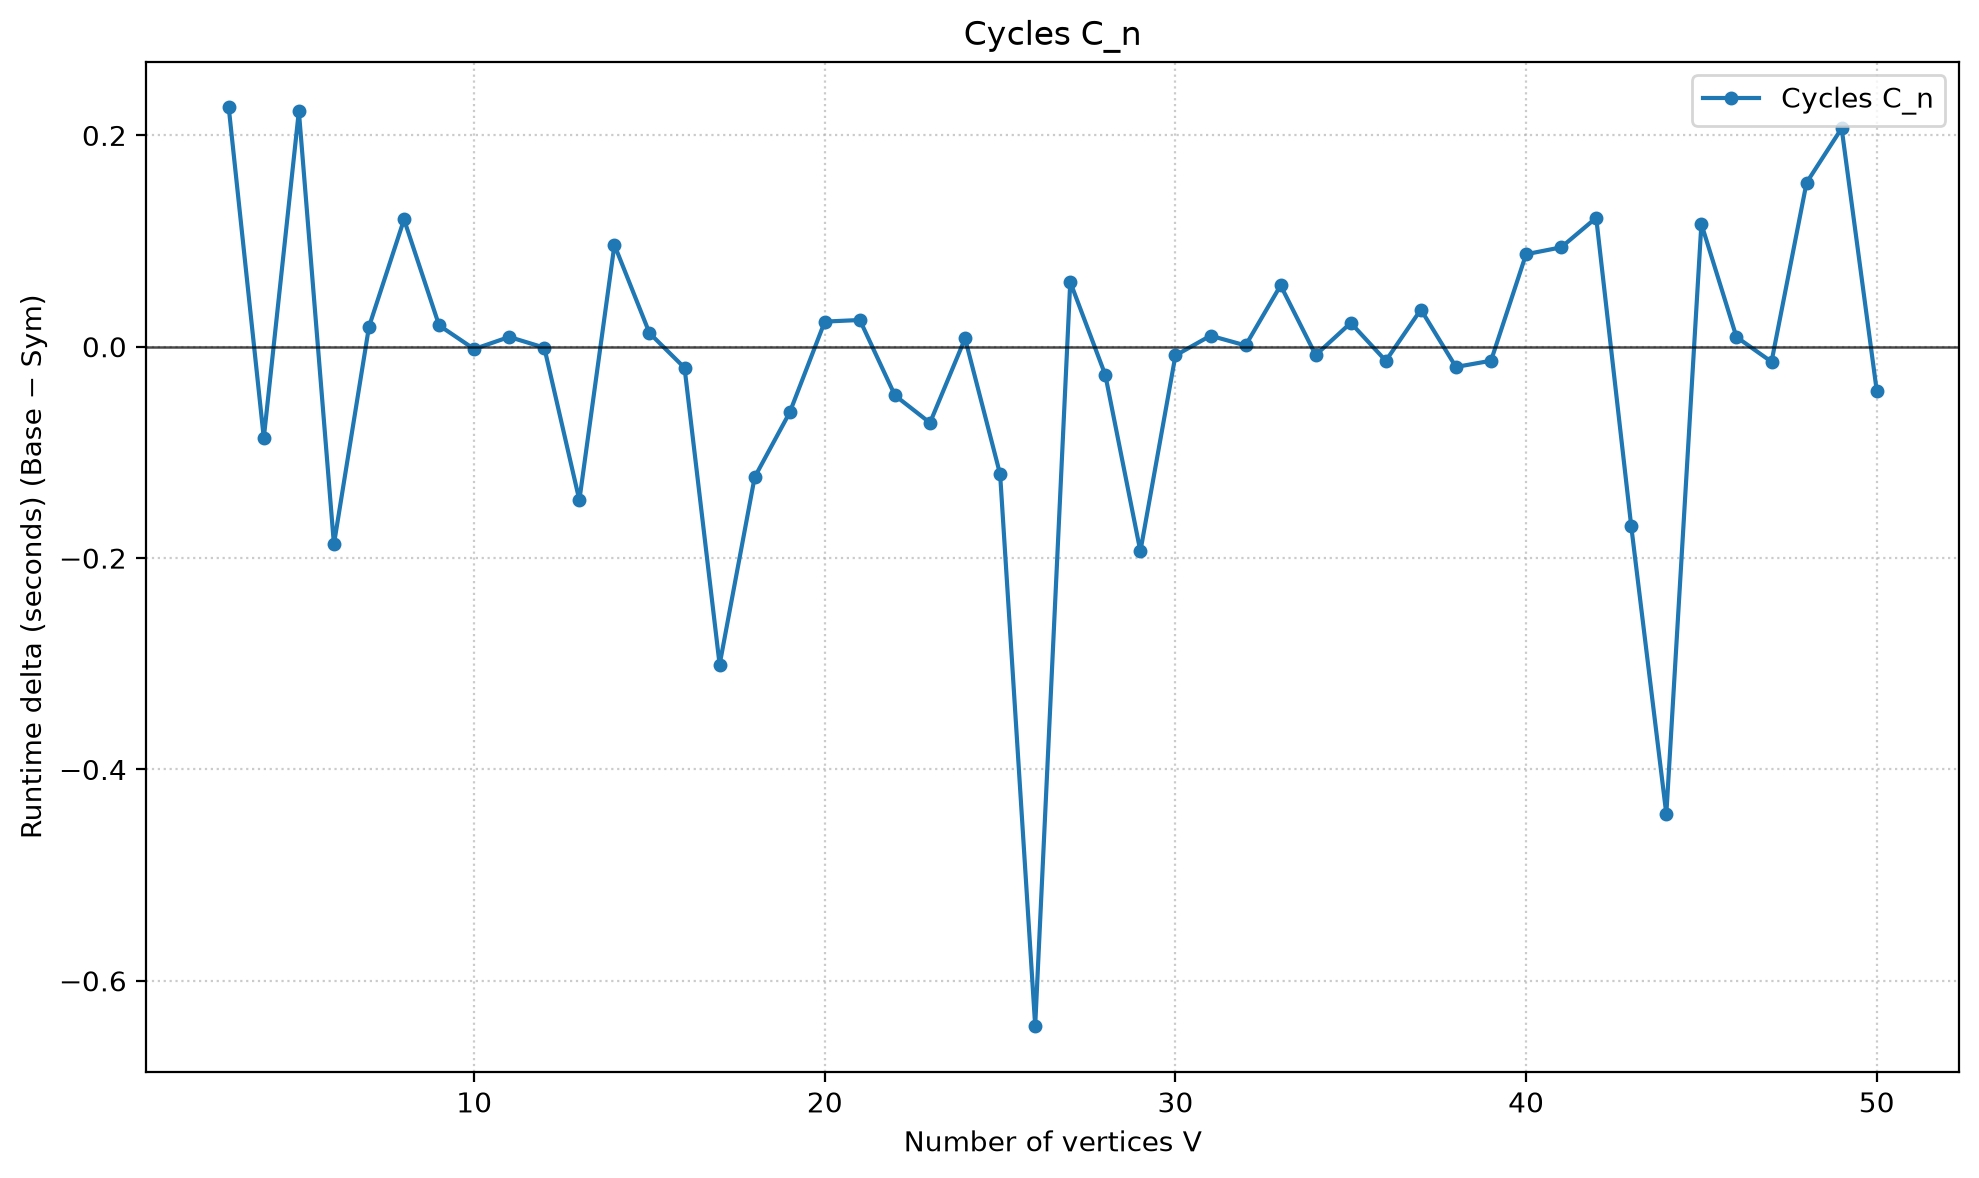
\includegraphics[width=0.49\linewidth]{paper/generated/cycles_main_r1_plots/delta_runtime_C.png}
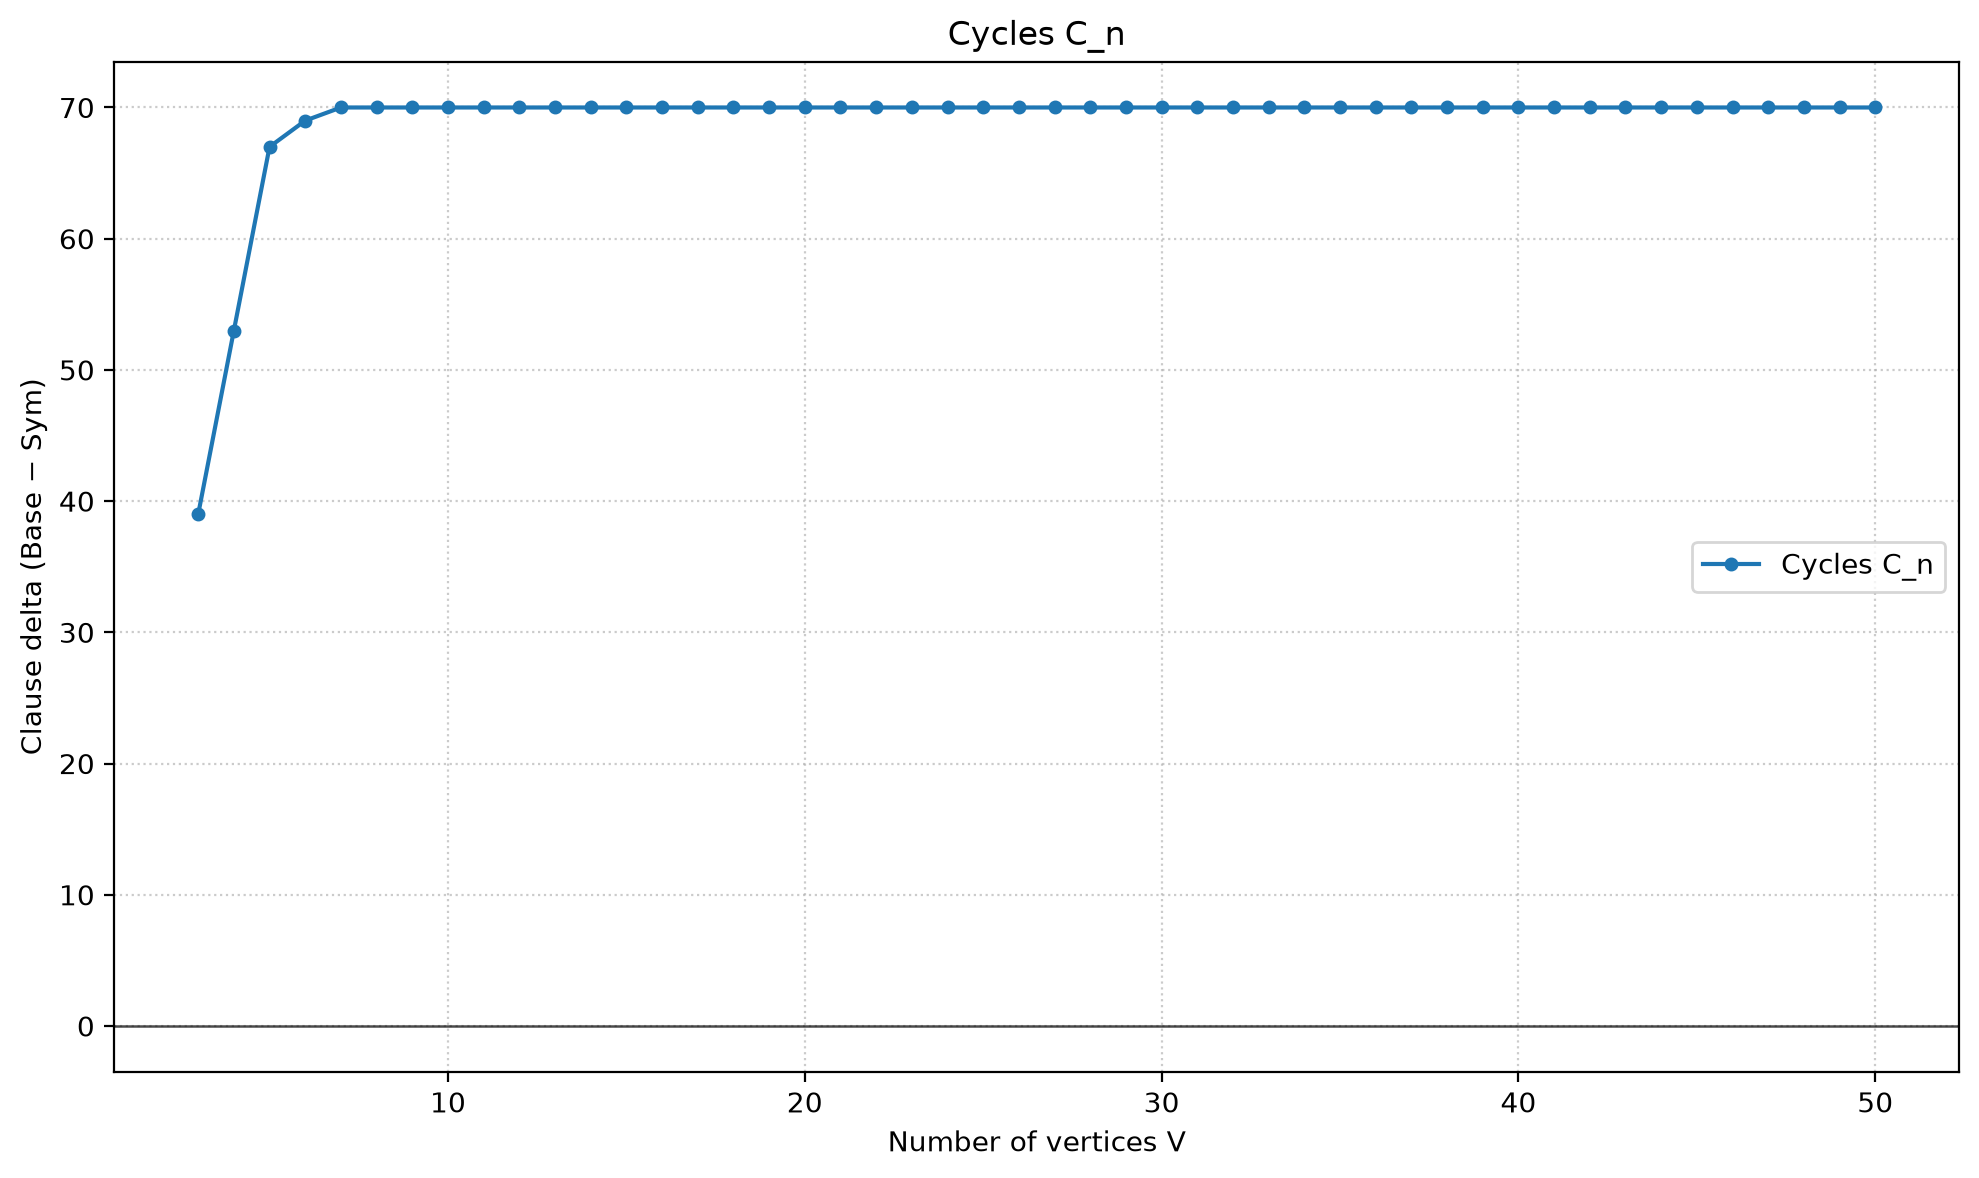
\includegraphics[width=0.49\linewidth]{paper/generated/cycles_main_r1_plots/delta_clauses_C.png}
\caption{Chu trình: chênh lệch runtime và số clause Base trừ Sym. Giá trị
âm ở hình thời gian nghĩa là lượt Symmetry chậm hơn.}
\end{figure}
\begin{figure}[htbp]
\centering
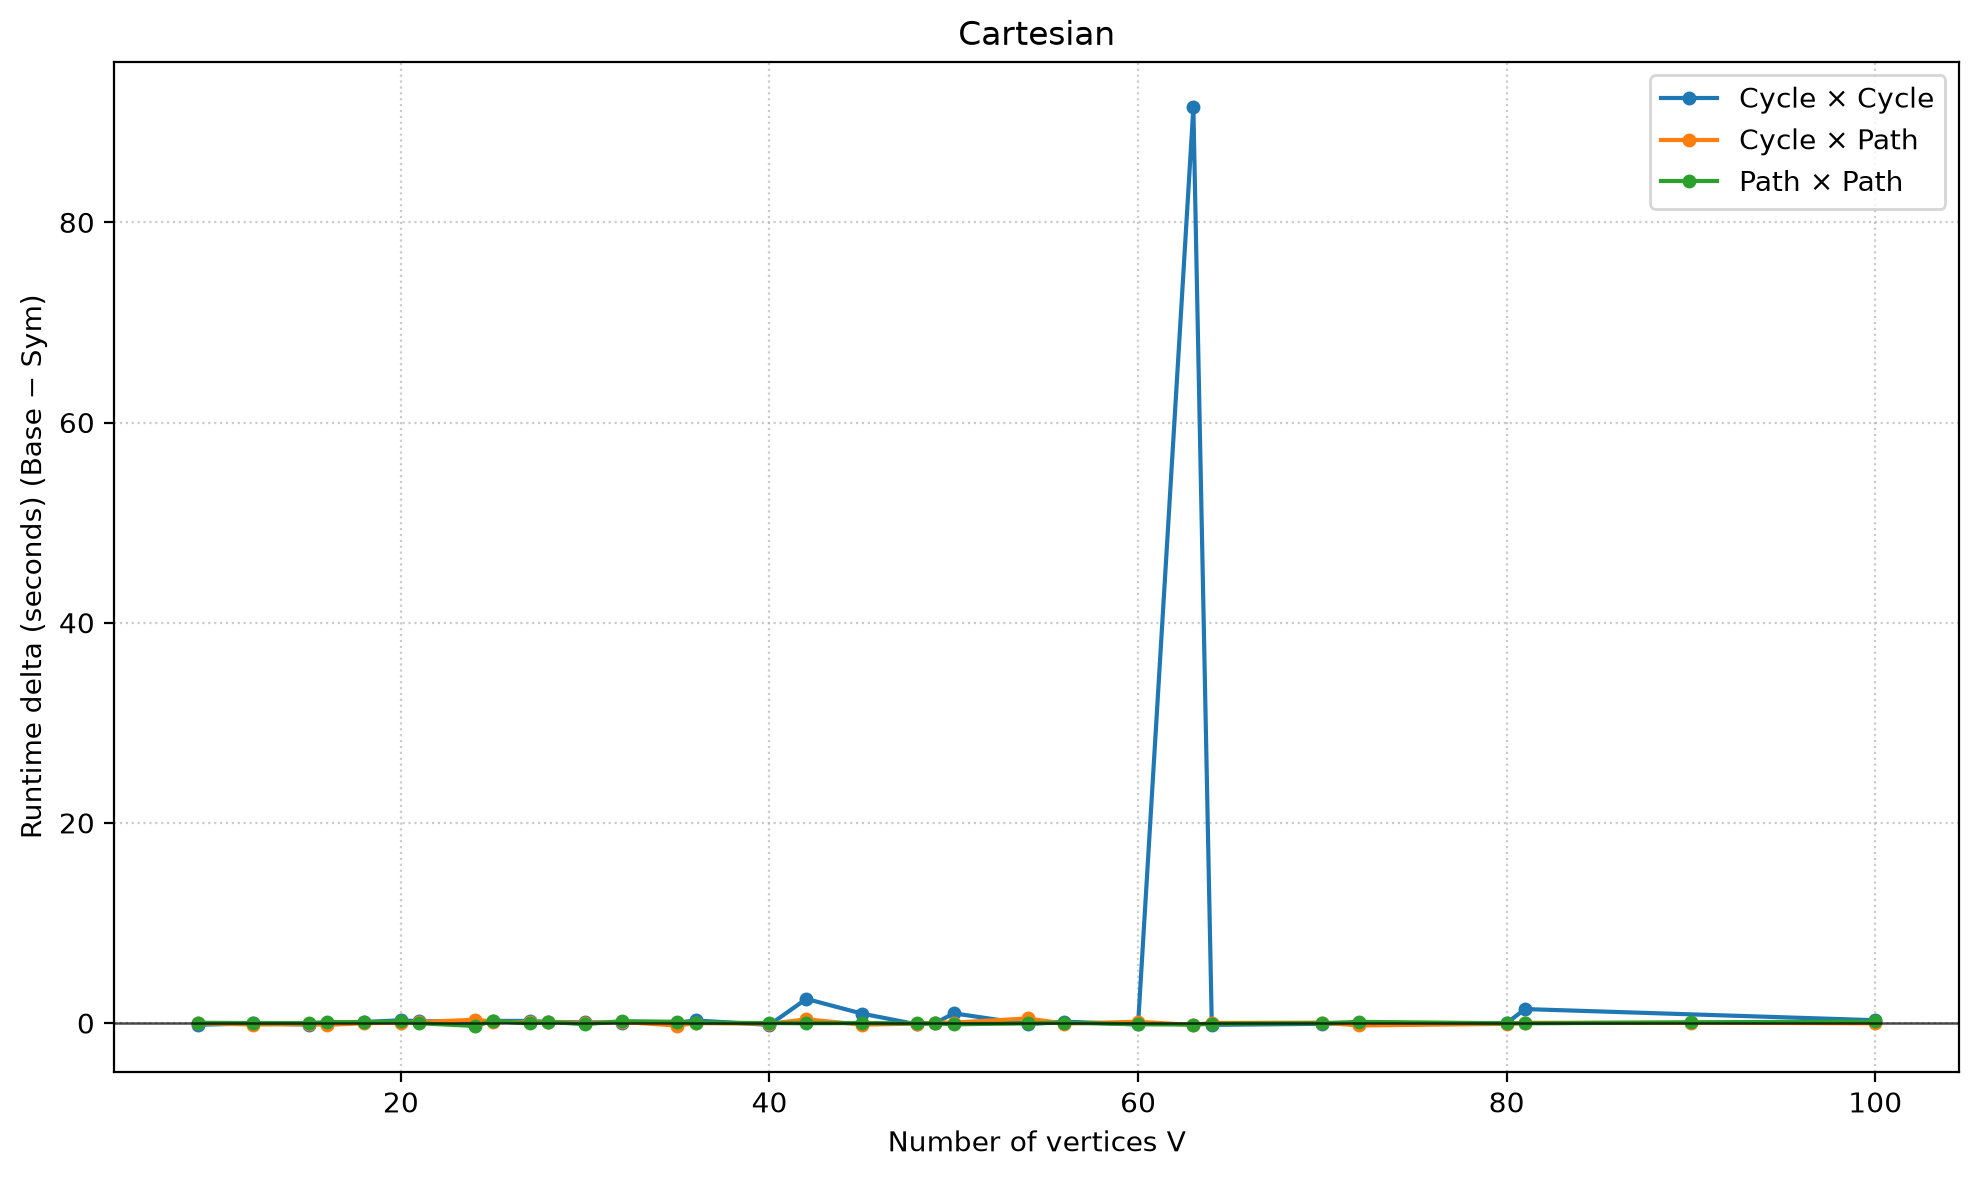
\includegraphics[width=0.49\linewidth]{paper/generated/products_main_r1_plots/delta_runtime_cartesian.png}
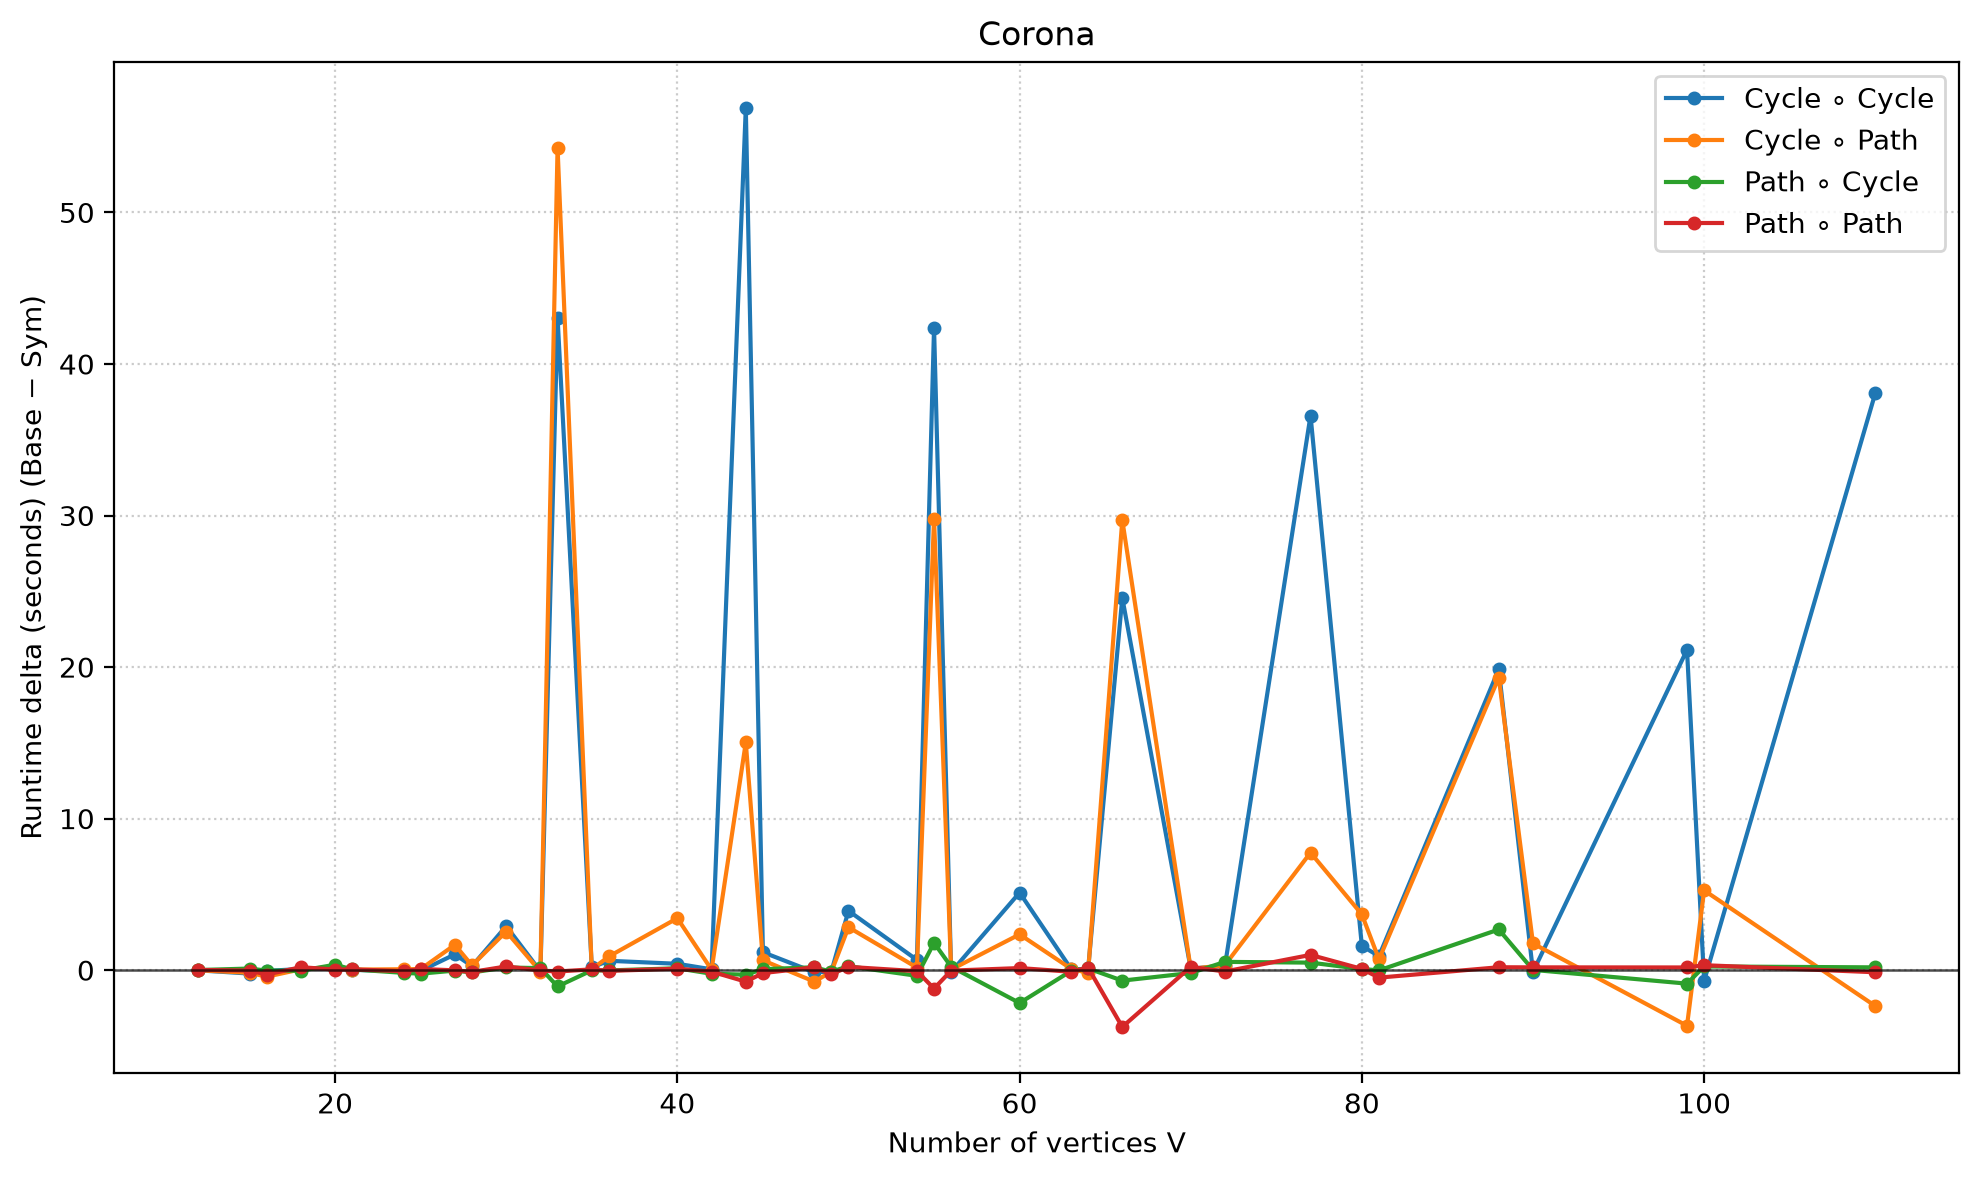
\includegraphics[width=0.49\linewidth]{paper/generated/products_main_r1_plots/delta_runtime_corona.png}
\caption{Runtime product: mỗi đường là một họ riêng, mỗi điểm là trung bình
chênh lệch trên các cặp cùng họ, cùng số đỉnh và cùng OPT. Không gộp các họ
thành một đường trung bình; hai cặp chưa tối ưu không nằm trong hình này.}
\end{figure}
\begin{figure}[htbp]
\centering
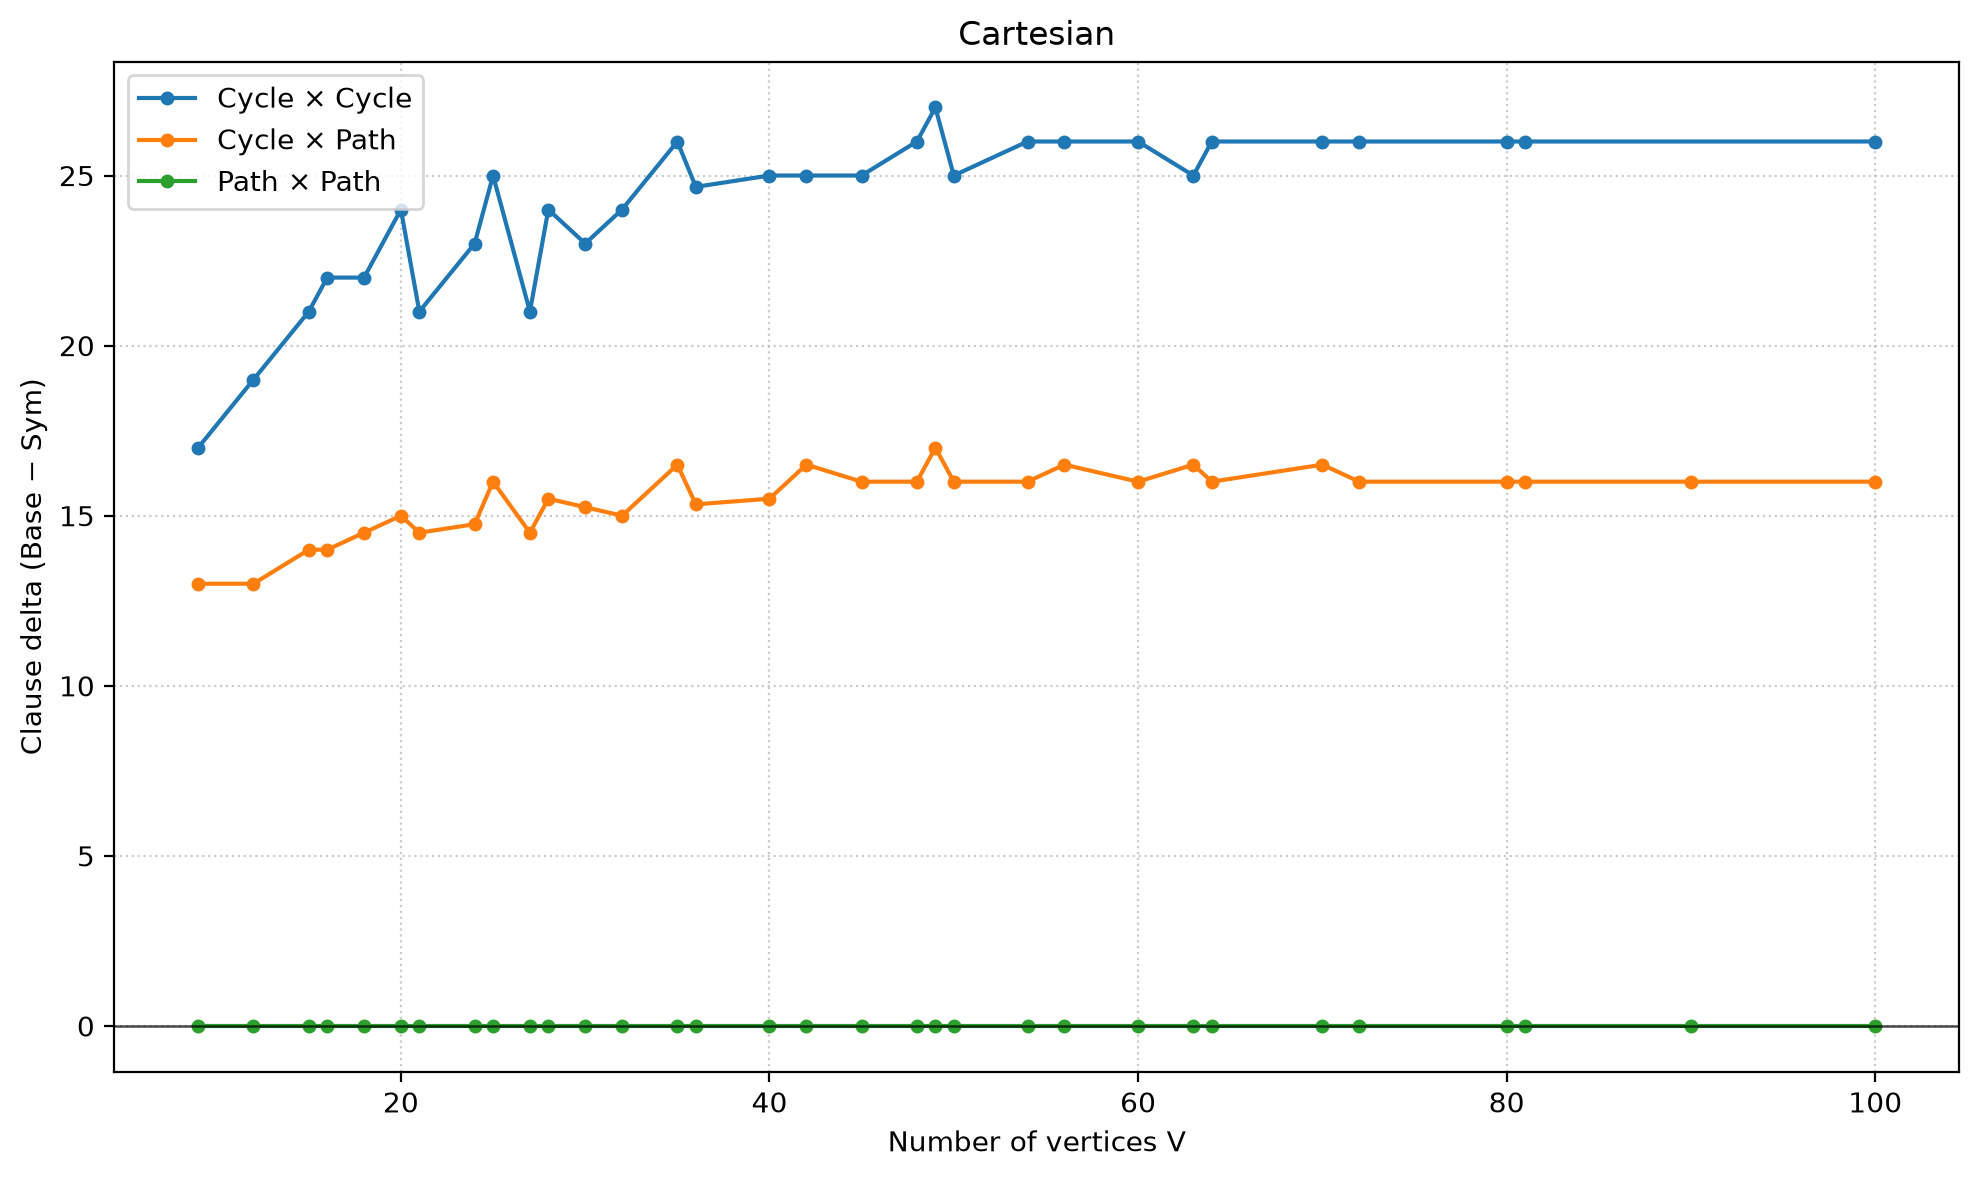
\includegraphics[width=0.49\linewidth]{paper/generated/products_main_r1_plots/delta_clauses_cartesian.png}
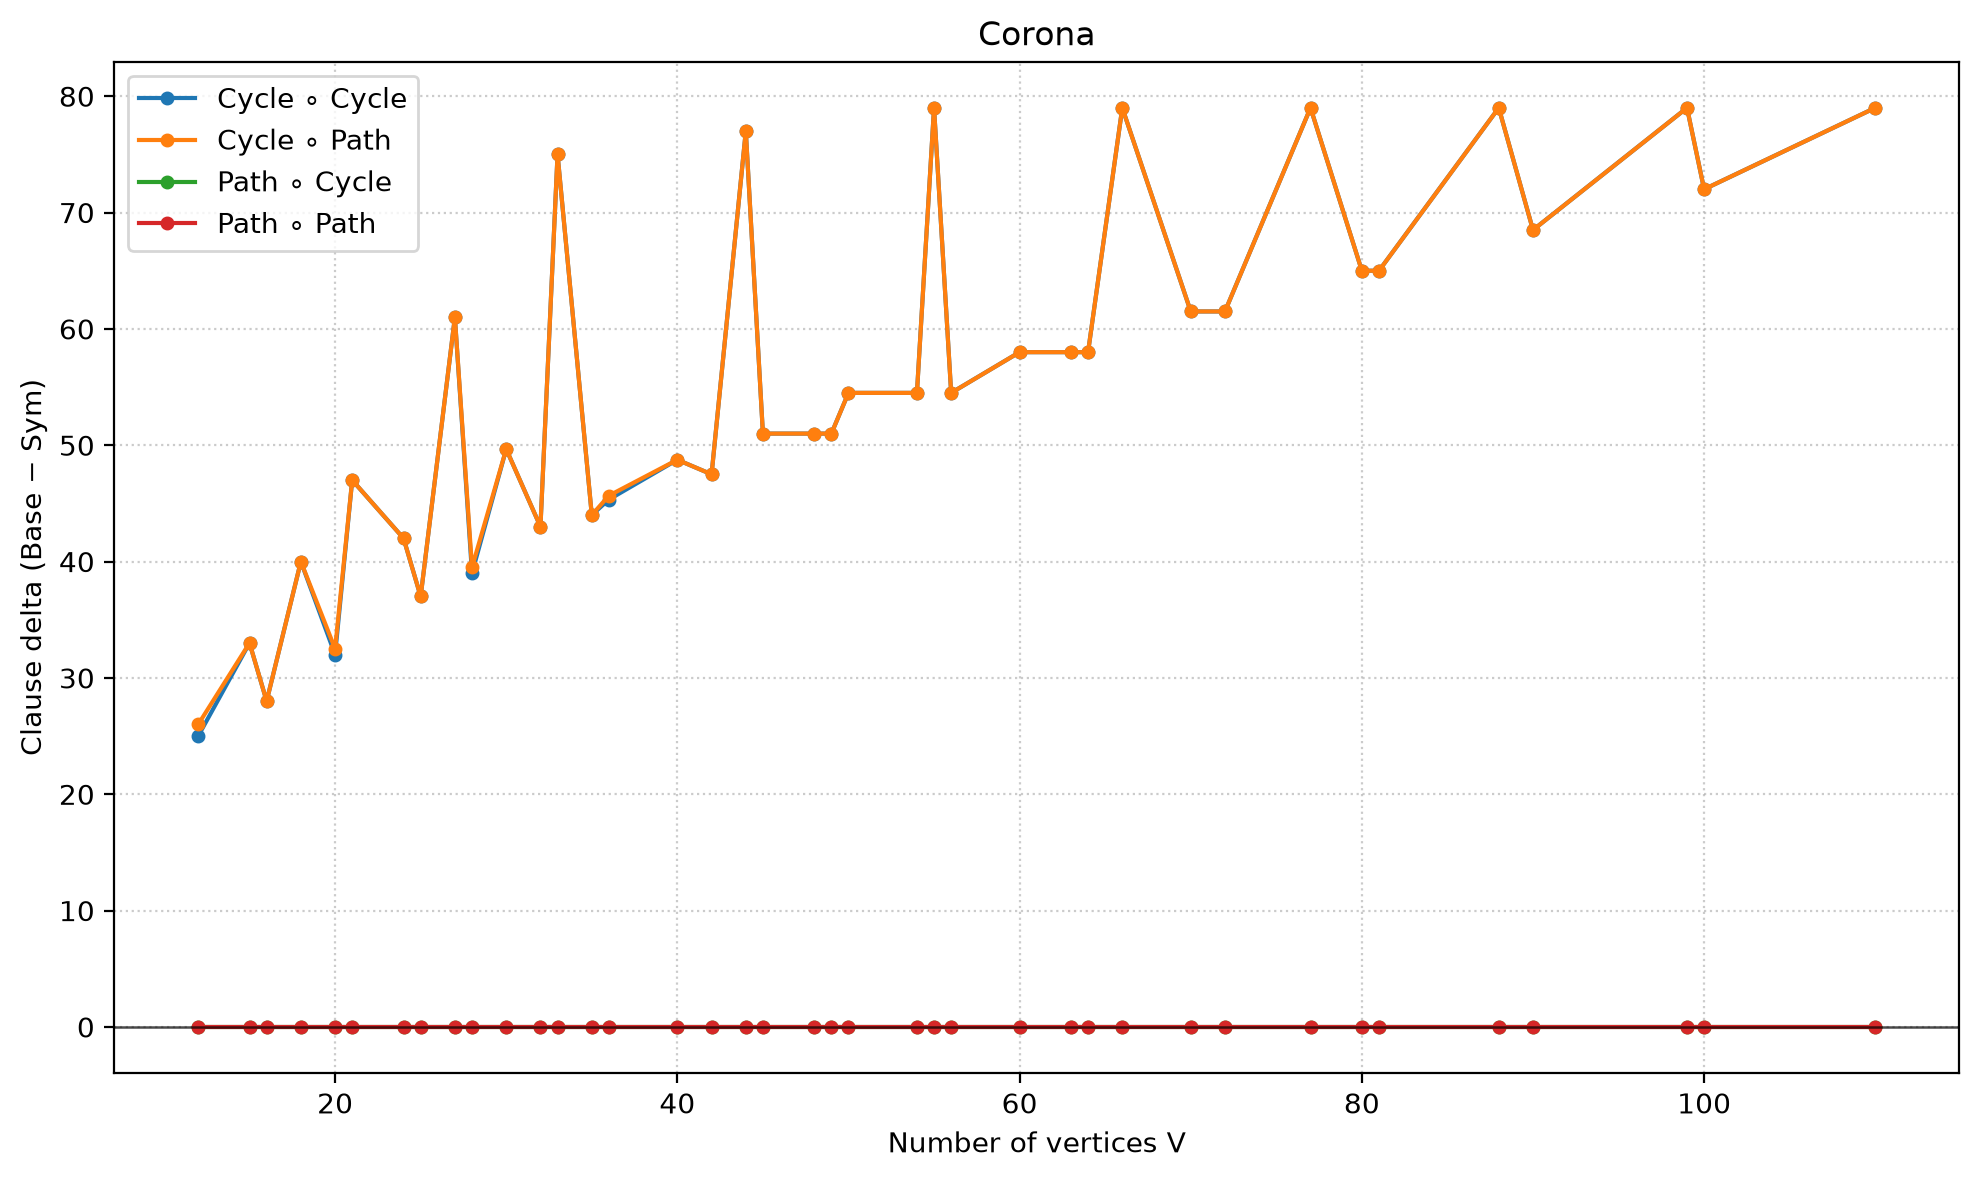
\includegraphics[width=0.49\linewidth]{paper/generated/products_main_r1_plots/delta_clauses_corona.png}
\caption{Clause product: Base trừ Sym tại cùng span, sau cùng tiền xử lý,
trên tập cặp OPT/OPT. Các đường giá trị 0 có thể trùng nhau ở những họ không
thêm điều kiện đối xứng riêng.}
\end{figure}
\FloatBarrier

\subsection{Bộ đếm tìm kiếm và thời gian thành phần}
\begin{table}[H]
\centering\small\setlength{\tabcolsep}{4pt}% Generated from main runs; do not edit numbers manually.
\begin{tabular}{lrrrr}
\toprule
Họ & Xung đột B & Xung đột S & Quyết định B & Quyết định S \\
\midrule
$C_n$ & 490 & 16 & 1014 & 304 \\
$C_n \mathbin{\square} C_m$ & 2822176 & 1561898 & 3703052 & 2086601 \\
$C_n \mathbin{\square} P_m$ & 62458 & 56542 & 96318 & 87201 \\
$P_n \mathbin{\square} P_m$ & 8282 & 8282 & 15175 & 15175 \\
$C_n \circ C_m$ & 28922138 & 19787058 & 35712056 & 24679416 \\
$C_n \circ P_m$ & 25550270 & 21037672 & 31640833 & 26452185 \\
$P_n \circ C_m$ & 15624199 & 15624199 & 19374024 & 19374024 \\
$P_n \circ P_m$ & 17120804 & 17120804 & 21294514 & 21294514 \\
\bottomrule
\end{tabular}

\caption{Tổng xung đột và quyết định của Glucose qua các lần thử span đã
hoàn tất, chỉ trên cặp OPT/OPT. Bao gồm cả lần thử SAT và UNSAT.}
\end{table}
\begin{table}[H]
\centering\small% Generated from main runs; do not edit numbers manually.
\begin{tabular}{lrrrr}
\toprule
Họ & Dựng CNF B & Dựng CNF S & SAT B & SAT S \\
\midrule
$C_n$ & 0.0033 & 0.0027 & 0.0001 & 0.0000 \\
$C_n \mathbin{\square} C_m$ & 0.0718 & 0.0652 & 0.0241 & 0.0143 \\
$C_n \mathbin{\square} P_m$ & 0.0551 & 0.0558 & 0.0076 & 0.0069 \\
$P_n \mathbin{\square} P_m$ & 0.0454 & 0.0443 & 0.0012 & 0.0011 \\
$C_n \circ C_m$ & 0.0661 & 0.0629 & 0.3988 & 0.2334 \\
$C_n \circ P_m$ & 0.0629 & 0.0605 & 0.4020 & 0.2809 \\
$P_n \circ C_m$ & 0.0642 & 0.0740 & 0.0628 & 0.0683 \\
$P_n \circ P_m$ & 0.0647 & 0.0531 & 0.0808 & 0.1007 \\
\bottomrule
\end{tabular}

\caption{Trung vị thời gian dựng CNF và thời gian bên trong lời gọi SAT
(giây), cộng theo từng quá trình tìm kiếm rồi lấy trung vị trên cặp OPT/OPT.}
\end{table}
Số clause ở một span chung đo kích thước mô hình; tổng quyết định/xung đột
đo công việc qua toàn bộ các span đã thử. Hai cấu hình có thể đi qua những
span khác nhau khi tìm được incumbent khác nhau; do đó không diễn giải
bộ đếm tổng thành hiệu năng của một lời gọi tại span cố định. Bộ đếm đầy đủ
ở các lượt OPT hỗ trợ phân tích tìm kiếm nhưng không tự thay thế phép đo
runtime hoặc các lượt lặp. Các bộ đếm khác backend cũng không được mặc
nhiên coi là cùng thước đo.

\subsection{Tái lập và giới hạn kiểm chứng}
Lệnh \texttt{make report} kiểm tra hai CSV cùng manifest/witness, dựng lại
counts, sinh bảng, sinh hình rồi biên dịch bản thảo. Các file kết quả gốc
không bị sửa. Resume của benchmark chỉ nhận cùng cấu hình, source, schema
và môi trường; muốn đổi budget hoặc thử lại dòng FEASIBLE phải tạo lượt mới.

Bộ kiểm thử dùng oracle vét cạn trên mọi đồ thị atlas đến 5 đỉnh, kiểm tra
mọi phép gán trên đồ thị 3 đỉnh, các giá trị $h,k$ ở mức encoder, tính tương
đương của rút gọn, phản xạ của các constructor và các ràng buộc ILP. Hai
kiểm thử tích hợp ILP chưa qua vì giới hạn runtime/license trong môi trường
kiểm tra. Vì vậy bản thảo này không đưa ra kết luận SAT nhanh hơn ILP.
Hai lượt main\_r1 là một lần đo mỗi cấu hình trên mỗi instance; chưa có
ước lượng phương sai hoặc khoảng tin cậy. Chọn riêng các cặp OPT/OPT có
thể thiên về instance dễ, nên các bảng thời gian không đại diện toàn bộ
miền khi vẫn còn cặp timeout.

\section{Diễn giải kết quả và hướng phát triển}
\subsection{Điều có thể kết luận từ lượt main\_r1}
Hai bộ dữ liệu hoàn chỉnh theo miền quét cho phép đối chiếu mô hình và
quan sát tác động của phá đối xứng trên cùng backend/cấu hình tìm kiếm.
Các nhãn đã được kiểm tra lại; các cặp cùng OPT không bất đồng span.
Tuy nhiên, giảm không gian nghiệm không đồng nghĩa giảm số clause theo
cùng tỉ lệ, và giảm clause không tự suy ra giảm thời gian tổng. Kết quả
chu trình cùng các họ product minh họa rõ sự khác nhau giữa ba đại lượng.

Cấu hình hiện tại cố ý chỉ cố định gốc trên $C_n$. Trên product, điều kiện
thứ tự dựa trên một phản xạ cụ thể chỉ khai thác một phần đối xứng của đồ
thị. Mức giảm clause nhỏ là kết quả của cấu hình đang được đánh giá, không
phải giới hạn lý thuyết của mọi phương pháp phá đối xứng trên họ đó. Các
họ chưa có ràng buộc riêng phải được nhận diện rõ như những lượt lặp cùng
mô hình. Không đưa thêm cố định gốc hoặc nhiều thứ tự đồng thời nếu chưa
chứng minh chúng cùng bảo toàn ít nhất một nghiệm trong mỗi lớp cần xét.

\subsection{Kết quả đã biết và quy luật hữu hạn}
Survey \cite{calamoneri} đã dẫn các kết quả chính xác cho tích của đường đi
và chu trình. Các giá trị quan sát trên Cartesian đóng vai trò đối chứng;
không gọi một quy luật là mới chỉ vì nó xuất hiện trong CSV. Điều kiện
tham số và các trường hợp nhỏ phải được đối chiếu với từng định lý gốc.

Trong lượt product main\_r1, có \CoronaPathMatches{} trên
\CoronaPathCount{} cặp đã xác nhận tối ưu của $C_n\circ P_m$ thỏa
\[
\lambda_{2,1}(C_n\circ P_m)=m+4.
\]
Đây là quan sát trên miền tham số đã quét. Để phát biểu cho mọi $n,m$, cần
đối chiếu tài liệu và chứng minh cả cận dưới lẫn construction đạt cận trên.
Cận bậc $\Delta+1=m+3$ chưa đủ để kết luận công thức trên. Ghi chú nghiên
cứu về Corona không phải bằng chứng rằng chưa có công trình giải quyết
bài toán. Hai instance Cartesian chưa tối ưu cần được khảo sát riêng;
incumbent của chúng không được đưa vào suy công thức tối ưu.

\subsection{Phần còn thiếu và bước tiếp theo}
Ưu tiên thực nghiệm là lặp lại các lượt với thứ tự Base/Sym được đảo cân
bằng, giữ nguyên máy, source và cấu hình để đo biến thiên. Với hai cặp
chưa tối ưu, có thể tạo lượt kiểm tra riêng với budget lớn hơn hoặc backend
khác; không ghép thời gian của lượt bổ sung vào bảng Glucose hiện tại như
cùng điều kiện đo. Để tách tác động của cố định gốc và phản xạ trên chu
trình, cần thêm các cấu hình ablation tương ứng.

Các bước phương pháp gồm chứng thư UNSAT độc lập; điều kiện phá đối xứng
mạnh hơn có chứng minh cho từng họ; SAT gia tăng qua assumptions/tái sử
dụng learned clauses; và đối chứng SAT--ILP trên cùng tập instance khi
backend ILP hoạt động. Project hiện chưa triển khai thuật toán chuyên biệt
trên cây, nên hướng đối chiếu với thuật toán đó vẫn là công việc tiếp theo.
Phần Petersen trong mô hình và tài liệu xác định phạm vi đồ thị; dữ liệu
lịch sử của nó chưa được đưa vào kết quả chính main\_r1.

Đóng góp được hỗ trợ bởi dữ liệu hiện tại là một quy trình mô hình hóa,
tìm kiếm tối ưu, áp dụng đối xứng có điều kiện, kiểm tra nhãn và đo thực
nghiệm có thể truy nguyên. Các kết luận về công thức tổng quát, mức độ mới
của kết quả toán học và độ ổn định của lợi ích hiệu năng còn cần chứng minh
hoặc thực nghiệm bổ sung tương ứng.

\bibliographystyle{plain}
\bibliography{paper/references}
\end{document}
